\documentclass[tikz,border=5pt]{standalone}
\pdfinfoomitdate=1
\pdftrailerid{}
\pdfsuppressptexinfo=-1
\usepackage{pgfplots}
\usepgfplotslibrary{groupplots}
\pgfplotsset{compat=1.18}
\pgfplotsset{colormap/viridis}
\definecolor{atlas0}{HTML}{0072B2}
\definecolor{atlas1}{HTML}{D55E00}
\definecolor{atlas2}{HTML}{009E73}
\definecolor{atlas3}{HTML}{E69F00}
\definecolor{atlas4}{HTML}{56B4E9}
\definecolor{atlas5}{HTML}{CC79A7}
\definecolor{atlas6}{HTML}{000000}
\definecolor{atlas7}{HTML}{F0E442}
% NATO SERS figure F13; data_sha256=111961c37f2c4337c66bbe694743de691c3c285b05d1904fac6d1ec261ec333b
% caption=(S) RQ-P01 within-station classical benchmark. Each mark is one complete four-fold pooled endpoint for one technical split repeat; spectrum and instrument-balanced master aggregation are separate. Marks at -0.05 denote terminally unavailable endpoints, not zero accuracy. The black dash-dot line is three-class chance (1/3). Ranges across repeats are descriptive because repeats are not independent samples. PP-U-MIN on the frozen 598-spectrum/69-master primary population.
\begin{document}
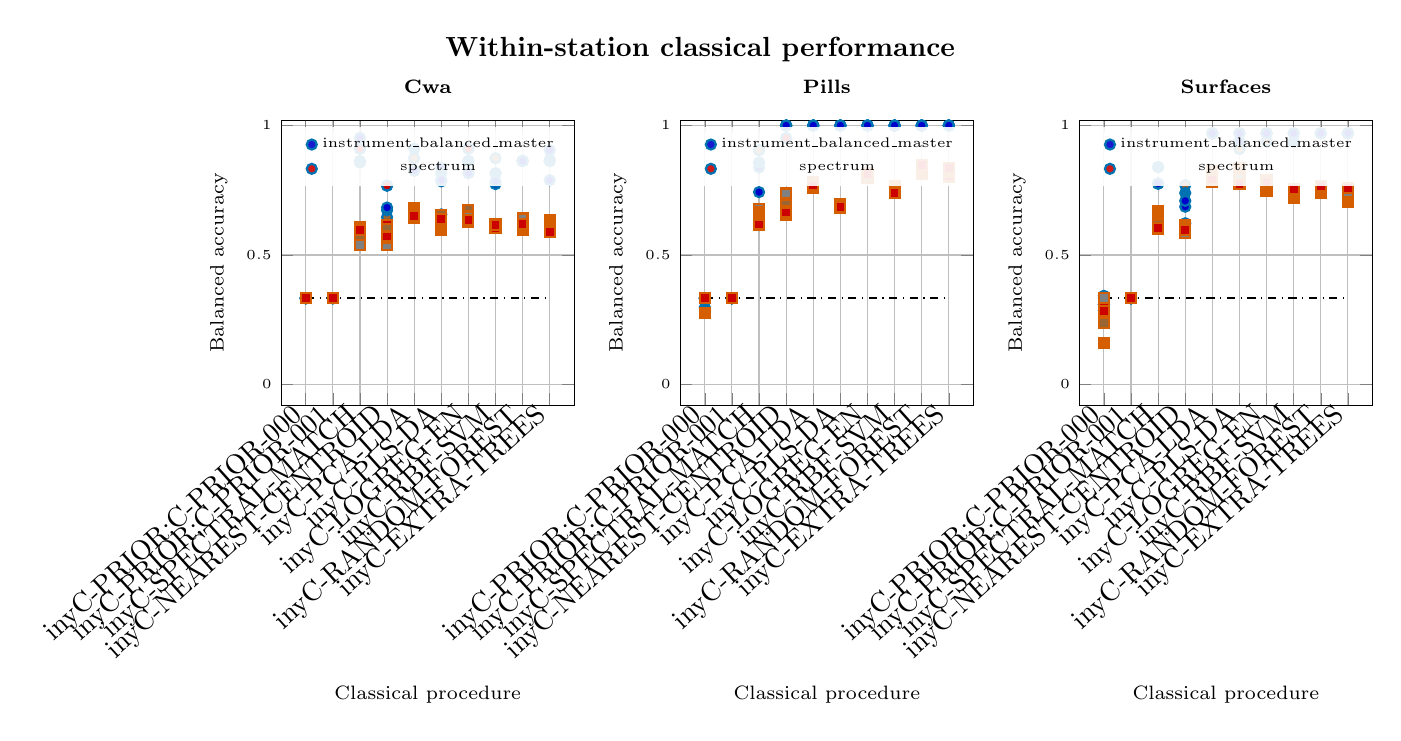
\begin{tikzpicture}
\begin{groupplot}[group style={group size=3 by 1, horizontal sep=1.35cm, vertical sep=1.5cm}, width=5.30cm, height=5.2cm, grid=major, tick label style={font=\tiny}, label style={font=\scriptsize}, title style={font=\scriptsize\bfseries,align=center}, legend style={font=\tiny,draw=none,fill=white,fill opacity=0.9,text opacity=1}]
\nextgroupplot[title={Cwa},xlabel={Classical procedure},ylabel={Balanced accuracy},ymin=-0.08,ymax=1.02,xtick={0,1,2,3,4,5,6,7,8,9},xticklabels={C-PRIOR:C-PRIOR-000,C-PRIOR:C-PRIOR-001,C-SPECTRAL-MATCH,C-NEAREST-CENTROID,C-PCA-LDA,C-PLS-DA,C-LOGREG-EN,C-RBF-SVM,C-RANDOM-FOREST,C-EXTRA-TREES},x tick label style={rotate=42,anchor=east,font=	iny}]
\addplot+[color=atlas0,mark=*,mark size=1.8pt,line width=0.8pt,only marks] coordinates {(0,0.33333333) (1,0.33333333) (2,0.91071429) (3,0.76785714) (4,0.8260582) (5,0.83664021) (6,0.91071429) (7,0.77380952) (8,0.86309524) (9,0.9047619)};
\addlegendentry{instrument\_balanced\_master}
\addplot+[color=atlas0,mark=*,mark size=1.8pt,line width=0.8pt,only marks] coordinates {(0,0.33333333) (1,0.33333333) (2,0.91071429) (3,0.76785714) (4,0.8260582) (5,0.78439153) (6,0.91071429) (7,0.81547619) (8,0.86309524) (9,0.86772487)};
\addplot+[color=atlas0,mark=*,mark size=1.8pt,line width=0.8pt,only marks] coordinates {(0,0.33333333) (1,0.33333333) (2,0.85714286) (3,0.64616402) (4,0.87367725) (5,0.65674603) (6,0.86309524) (7,0.87367725) (8,0.86309524) (9,0.86309524)};
\addplot+[color=atlas0,mark=*,mark size=1.8pt,line width=0.8pt,only marks] coordinates {(0,0.33333333) (1,0.33333333) (2,0.86309524) (3,0.67261905) (4,0.91071429) (5,0.81547619) (6,0.86309524) (7,0.81547619) (8,0.86309524) (9,0.86309524)};
\addplot+[color=atlas0,mark=*,mark size=1.8pt,line width=0.8pt,only marks] coordinates {(0,0.33333333) (1,0.33333333) (2,0.95238095) (3,0.68320106) (4,0.8260582) (5,0.78902116) (6,0.81547619) (7,0.78439153) (8,0.86309524) (9,0.78902116)};
\addplot+[color=atlas1,mark=square*,mark size=1.8pt,line width=0.8pt,only marks] coordinates {(0,0.33333333) (1,0.33333333) (2,0.58103042) (3,0.61595502) (4,0.67619864) (5,0.63777639) (6,0.67070542) (7,0.60508545) (8,0.62208457) (9,0.61670822)};
\addlegendentry{spectrum}
\addplot+[color=atlas1,mark=square*,mark size=1.8pt,line width=0.8pt,only marks] coordinates {(0,0.33333333) (1,0.33333333) (2,0.57577096) (3,0.59998615) (4,0.65995273) (5,0.65522137) (6,0.67393469) (7,0.61579485) (8,0.63941267) (9,0.6270237)};
\addplot+[color=atlas1,mark=square*,mark size=1.8pt,line width=0.8pt,only marks] coordinates {(0,0.33333333) (1,0.33333333) (2,0.53980746) (3,0.53766038) (4,0.64195366) (5,0.60527592) (6,0.64896629) (7,0.61495507) (8,0.64076325) (9,0.62543071)};
\addplot+[color=atlas1,mark=square*,mark size=1.8pt,line width=0.8pt,only marks] coordinates {(0,0.33333333) (1,0.33333333) (2,0.60898568) (3,0.56545547) (4,0.67942791) (5,0.59643655) (6,0.62881149) (7,0.6183445) (8,0.59711617) (9,0.63431337)};
\addplot+[color=atlas1,mark=square*,mark size=1.8pt,line width=0.8pt,only marks] coordinates {(0,0.33333333) (1,0.33333333) (2,0.59580022) (3,0.57151144) (4,0.6509532) (5,0.63896681) (6,0.63578083) (7,0.61483819) (8,0.61846138) (9,0.58811663)};
\addplot[black,dashdotted,line width=0.7pt,forget plot] coordinates {(0,0.33333333) (9,0.33333333)};
\nextgroupplot[title={Pills},xlabel={Classical procedure},ylabel={Balanced accuracy},ymin=-0.08,ymax=1.02,xtick={0,1,2,3,4,5,6,7,8,9},xticklabels={C-PRIOR:C-PRIOR-000,C-PRIOR:C-PRIOR-001,C-SPECTRAL-MATCH,C-NEAREST-CENTROID,C-PCA-LDA,C-PLS-DA,C-LOGREG-EN,C-RBF-SVM,C-RANDOM-FOREST,C-EXTRA-TREES},x tick label style={rotate=42,anchor=east,font=	iny}]
\addplot+[color=atlas0,mark=*,mark size=1.8pt,line width=0.8pt,only marks] coordinates {(0,0.33333333) (1,0.33333333) (2,0.83809524) (3,1) (4,1) (5,1) (6,1) (7,1) (8,1) (9,1)};
\addlegendentry{instrument\_balanced\_master}
\addplot+[color=atlas0,mark=*,mark size=1.8pt,line width=0.8pt,only marks] coordinates {(0,0.33333333) (1,0.33333333) (2,0.9047619) (3,0.95238095) (4,1) (5,1) (6,1) (7,1) (8,1) (9,1)};
\addplot+[color=atlas0,mark=*,mark size=1.8pt,line width=0.8pt,only marks] coordinates {(0,0.33333333) (1,0.33333333) (2,0.9047619) (3,1) (4,1) (5,1) (6,1) (7,1) (8,1) (9,1)};
\addplot+[color=atlas0,mark=*,mark size=1.8pt,line width=0.8pt,only marks] coordinates {(0,0.29761905) (1,0.33333333) (2,0.85714286) (3,1) (4,1) (5,1) (6,1) (7,1) (8,1) (9,1)};
\addplot+[color=atlas0,mark=*,mark size=1.8pt,line width=0.8pt,only marks] coordinates {(0,0.33333333) (1,0.33333333) (2,0.74285714) (3,1) (4,1) (5,1) (6,1) (7,1) (8,1) (9,1)};
\addplot+[color=atlas1,mark=square*,mark size=1.8pt,line width=0.8pt,only marks] coordinates {(0,0.33333333) (1,0.33333333) (2,0.62770089) (3,0.65424714) (4,0.75836005) (5,0.69757213) (6,0.81562932) (7,0.75154104) (8,0.81386348) (9,0.80300779)};
\addlegendentry{spectrum}
\addplot+[color=atlas1,mark=square*,mark size=1.8pt,line width=0.8pt,only marks] coordinates {(0,0.33333333) (1,0.33333333) (2,0.65273868) (3,0.69301418) (4,0.7808794) (5,0.6817936) (6,0.81397099) (7,0.74650416) (8,0.82501238) (9,0.82970391)};
\addplot+[color=atlas1,mark=square*,mark size=1.8pt,line width=0.8pt,only marks] coordinates {(0,0.33333333) (1,0.33333333) (2,0.67812182) (3,0.73767821) (4,0.77196549) (5,0.68859632) (6,0.79956734) (7,0.74336344) (8,0.82587249) (9,0.81964644)};
\addplot+[color=atlas1,mark=square*,mark size=1.8pt,line width=0.8pt,only marks] coordinates {(0,0.27697957) (1,0.33333333) (2,0.66445448) (3,0.66951091) (4,0.77653322) (5,0.69242774) (6,0.81317278) (7,0.76652136) (8,0.82124286) (9,0.82130477)};
\addplot+[color=atlas1,mark=square*,mark size=1.8pt,line width=0.8pt,only marks] coordinates {(0,0.33333333) (1,0.33333333) (2,0.61758152) (3,0.66414497) (4,0.76813407) (5,0.68396669) (6,0.81397099) (7,0.74062345) (8,0.84707887) (9,0.83491021)};
\addplot[black,dashdotted,line width=0.7pt,forget plot] coordinates {(0,0.33333333) (9,0.33333333)};
\nextgroupplot[title={Surfaces},xlabel={Classical procedure},ylabel={Balanced accuracy},ymin=-0.08,ymax=1.02,xtick={0,1,2,3,4,5,6,7,8,9},xticklabels={C-PRIOR:C-PRIOR-000,C-PRIOR:C-PRIOR-001,C-SPECTRAL-MATCH,C-NEAREST-CENTROID,C-PCA-LDA,C-PLS-DA,C-LOGREG-EN,C-RBF-SVM,C-RANDOM-FOREST,C-EXTRA-TREES},x tick label style={rotate=42,anchor=east,font=	iny}]
\addplot+[color=atlas0,mark=*,mark size=1.8pt,line width=0.8pt,only marks] coordinates {(0,0.34242424) (1,0.33333333) (2,0.83939394) (3,0.68636364) (4,0.96969697) (5,0.93939394) (6,0.96969697) (7,0.96969697) (8,0.96969697) (9,0.96969697)};
\addlegendentry{instrument\_balanced\_master}
\addplot+[color=atlas0,mark=*,mark size=1.8pt,line width=0.8pt,only marks] coordinates {(0,0.30909091) (1,0.33333333) (2,0.77575758) (3,0.62272727) (4,0.96969697) (5,0.96969697) (6,0.96969697) (7,0.96969697) (8,0.96969697) (9,0.96969697)};
\addplot+[color=atlas0,mark=*,mark size=1.8pt,line width=0.8pt,only marks] coordinates {(0,0.33333333) (1,0.33333333) (2,0.77575758) (3,0.76969697) (4,0.96969697) (5,0.90909091) (6,0.93939394) (7,0.93636364) (8,0.96969697) (9,0.96969697)};
\addplot+[color=atlas0,mark=*,mark size=1.8pt,line width=0.8pt,only marks] coordinates {(0,0.28484848) (1,0.33333333) (2,0.83939394) (3,0.73939394) (4,0.96969697) (5,0.96969697) (6,0.96969697) (7,0.93636364) (8,0.96969697) (9,0.96969697)};
\addplot+[color=atlas0,mark=*,mark size=1.8pt,line width=0.8pt,only marks] coordinates {(0,0.30909091) (1,0.33333333) (2,0.77575758) (3,0.70909091) (4,0.96969697) (5,0.96969697) (6,0.96969697) (7,0.96969697) (8,0.96969697) (9,0.96969697)};
\addplot+[color=atlas1,mark=square*,mark size=1.8pt,line width=0.8pt,only marks] coordinates {(0,0.29849881) (1,0.33333333) (2,0.65928824) (3,0.58979308) (4,0.80052744) (5,0.80752333) (6,0.76238915) (7,0.72090071) (8,0.74256071) (9,0.72215267)};
\addlegendentry{spectrum}
\addplot+[color=atlas1,mark=square*,mark size=1.8pt,line width=0.8pt,only marks] coordinates {(0,0.23688634) (1,0.33333333) (2,0.61819394) (3,0.58500551) (4,0.78118588) (5,0.79641222) (6,0.78939895) (7,0.73202921) (8,0.75713209) (9,0.74091462)};
\addplot+[color=atlas1,mark=square*,mark size=1.8pt,line width=0.8pt,only marks] coordinates {(0,0.33333333) (1,0.33333333) (2,0.60057381) (3,0.58500551) (4,0.81115168) (5,0.79527039) (6,0.78883672) (7,0.74839738) (8,0.74083927) (9,0.72914855)};
\addplot+[color=atlas1,mark=square*,mark size=1.8pt,line width=0.8pt,only marks] coordinates {(0,0.15921869) (1,0.33333333) (2,0.6680983) (3,0.61555092) (4,0.82456384) (5,0.83748913) (6,0.74716281) (7,0.72090071) (8,0.74379528) (9,0.70625398)};
\addplot+[color=atlas1,mark=square*,mark size=1.8pt,line width=0.8pt,only marks] coordinates {(0,0.2844143) (1,0.33333333) (2,0.60410943) (3,0.59793079) (4,0.79181012) (5,0.77476961) (6,0.78000927) (7,0.75606561) (8,0.76783168) (9,0.75969397)};
\addplot[black,dashdotted,line width=0.7pt,forget plot] coordinates {(0,0.33333333) (9,0.33333333)};
\end{groupplot}
\node[font=\normalsize\bfseries,anchor=south] at (current bounding box.north) {Within-station classical performance};
\end{tikzpicture}
\end{document}
